\title{24. Trigonometrické řešení obecného trojúhelníka}
\author{Kateřina Polášková (Jakub Sláma)}
\date{30.4.2025}

\maketitle

\section{Trigonometrické řešení obecného trojúhelníka}
Pro řešení obecného trojúhelníka (tj. ne pravoúhlého) se používají trigonometrické věty: sinová a kosinová věta.
\subsection{Sinová věta}
Pro každý trojúhelník ABC, jehož vnitřní úhly mají velikost $\alpha, \beta, \gamma$ a strany velikost $a, b, c$ platí:
$$
    \frac{a}{\sin \alpha} = \frac{b}{\sin \beta} = \frac{c}{\sin \gamma} = 2r,
$$
kde r je poloměr kružnice opsané
\\ 
\\
Sinovou větu používáme při řešení trojúhelníku, jsou-li dány \\
a) velikosti jedné strany a dvou úhlů přilehlých (věta usu) \\
b) velikosti dvou stran a úhlu proti jedné z nich (věta ssu)
\subsection{Kosinová věta}
Pro každý trojúhelník ABC, jehož vnitřní úhly mají velikost $\alpha, \beta, \gamma$ a strany velikost $a, b, c$ platí:
$$
    a^2 = b^2 + c^2 - 2bc \cdot \cos\alpha
$$
$$
    b^2 = a^2 + c^2 - 2ac \cdot \cos\beta
$$
$$
    c^2 = a^2 + b^2 - 2ab \cdot \cos\gamma
$$
Kosinovou větu používáme při řešení trojúhelníků, jsou-li dány 
\\
a) velikosti všech tří stran (věta sss)\\
b) velikosti dvou stran a úhlu jimi sevřeného (věta sus)

\subsection{Euklidovy věty}  
\subsubsection{Euklidova věta o výšce}
V každém pravoúhlém trojúhelníku s odvěsnami $a, b$ s přeponou $c$ a výškou $k$ přeponě $v_c$ platí:\\
Obsah čtverce nad výškou pravoúhlého trojúhelníku je roven obsahu obdélníku sestrojeného z obou úseků přepony.

\begin{figure}[H]
        \centering
        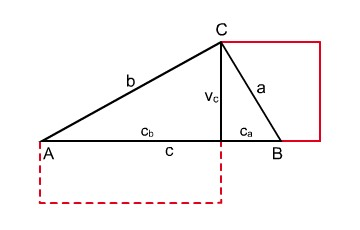
\includegraphics[width=0.5\linewidth]{img/24_euklidovy_vety.png}
        \caption{Euklidova věta o výšce} 
        \label{fig:enter-label}
    \end{figure}
$$
    v_c^2=c_a\cdot c_b
$$
\subsubsection{Euklidova věta o odvěsně}
V každém pravoúhlém trojúhelníku s odvěsnami a, b a s přeponou c platí:
Obsah čtverce sestrojeného nad odvěsnou pravoúhlého trojúhelníku je roven obsahu obdélníku sestrojeného z přepony a přilehlého úseku.
\begin{figure}[H]
        \centering
        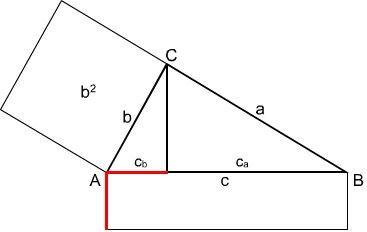
\includegraphics[width=0.5\linewidth]{img/24_euklidovy_vety_2.png}
        \caption{Euklidova věta o odvěsně} 
        \label{fig:enter-label}
    \end{figure}

$$
    b^2=c \cdot c_b
$$

\begin{figure}[H]
        \centering
        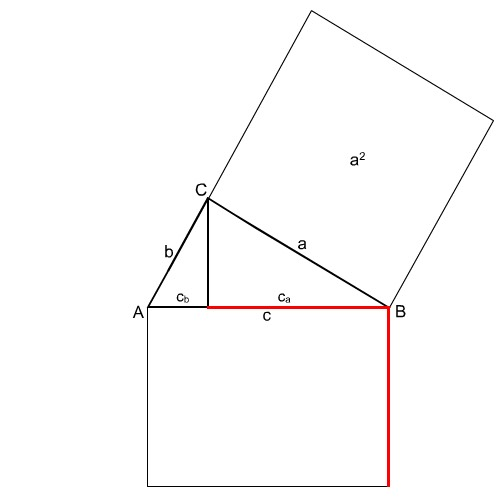
\includegraphics[width=0.5\linewidth]{img/24_euklidovy_vety_3.png}
        \caption{Euklidova věta o odvěsně} 
        \label{fig:enter-label}
    \end{figure}

$$
    a^2=c \cdot c_a
$$